\documentclass[a4paper,12pt]{article}
\usepackage[utf8]{inputenc}
\usepackage[dvipsnames]{xcolor}
\usepackage{graphicx}
\usepackage{tikz}
\usepackage[export]{adjustbox}
\usepackage[margin=0.4in]{geometry}
\usepackage{fancyhdr}
\usepackage{xcolor}
\usepackage{colortbl}
\usepackage{hyperref}
\usepackage{color,soul}

\setlength{\parindent}{0pt}
\setlength{\parskip}{5pt plus 1pt}
\setlength{\headheight}{13.6pt}



\begin{document}

\begin{center}

{\Huge\textsf{\underline{Electrical Engineer's Resources.}}}
\end{center}

\vspace{0.7in}



Hi, I am \textbf{Adhithya} from 3rd Year (2020-2024) EEE A Rajalakshmi Engineering college.
\begin{center}
\fbox{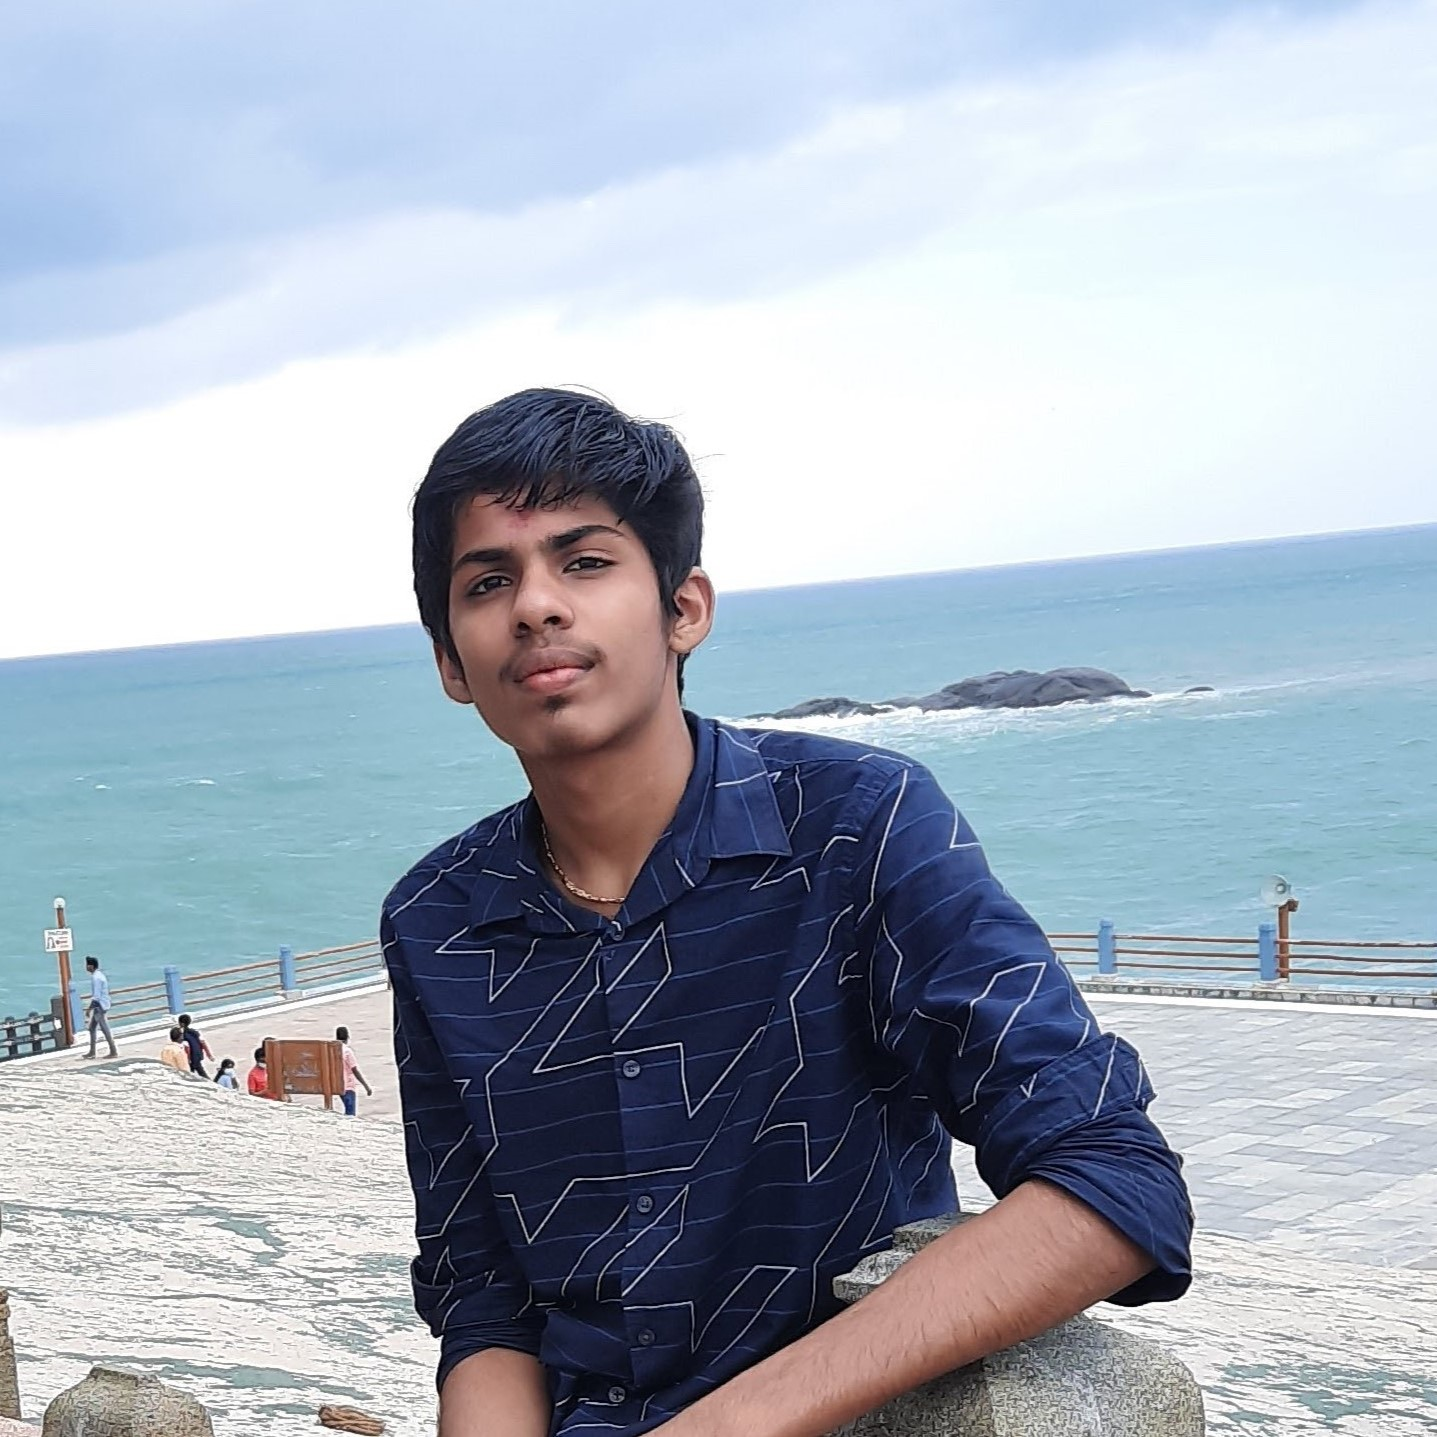
\includegraphics[width=2.5in]{adhithya.jpg}}
\end{center}
And that's me, I would like to share some tips and resources that I collected till date to you.

Electrical engineering is arguably the most wonderful field, Ohh the satisfaction you gain cannot be described by words...


\section{Question you might have}


\textit{Now that I have chosen electrical engineering}
\begin{enumerate}
\item \textit{``Does it have scope?''}
\item \textit{``Will I like it?''}
\item \textit{``Are the subjects difficult?''}
\end{enumerate}

Answer to all that is Big {\large\textbf{YES}} except for the last question, which is subjective.

But I can assure you, If start to love the subjects then nothing will be difficult.

Nothing you study in these 4 years will be useless. Bare that in mind. 

\textit{Why do I have to study chemistry? }

Because for eg. in steam power plants boilers have problem of forming scale and sludge to get overview what's happening in the plant you have to study it. You don't wanna be blank when the chemical engineers are fixing the problem. 

\textit{Why do I have to study linear algebra?}

In your fifth-sem you will be studying a subject called Power system analysis, There all the matrix manipulation you study here will be extensively used.


\vspace{1in}


\section{Tips from my experience.}
\begin{enumerate}
    \item Get a decent laptop if you don't have. (i5 processor is minimum, 8 GB RAM, 2/4GB Graphics card.)
    
    \item Get used to studying in laptop with ebooks/.pdf. Since you cannot buy every book.
    
    \item\textbf{Don't use} local author books, Like the books that say``Revised by Anna university syllabus''(Technical publications/Bakshi/Anuradha etc...), 

    The reason is no-one know who/what is correct, they most of the time confuse you and will make you to think subject is hard/difficult while in reality the book is poorly written. Same goes for Indian author books. Mostly try to avoid them, There are almost always better foreign author book.

    \item Never study for marks, Always remember to ask yourself {\large{Why?}} should I do like this? What this formula is saying? Why the concept is the the way it is? Trust me you will thank me later. Because electrical engineering's curriculum is framed in such a way that one concept is built on top of other. If you try to skip one thing it will rub-off on you later. 

    I should admit understanding math is difficult. but doing math without knowing anything just plugging in numbers and getting answers anyone can do you don't need an Engineering degree for that. Engineers are expected to understand concepts and apply them in real life for a problem which has not yet been solved.

    Most colleges don't make these kind of engineers and that is why very little to 0 electrical companies are coming for placement.


\end{enumerate}

\section{Useful Resources}

{\Large{\textbf{My website}}}

I created this website to condense all the resources, It contains books/Youtube video others to understand concepts

\url{{https://200901002.github.io/ee}} 

\vspace{0.2in}

Useful website apps/ YT channels

\url{{https://200901002.github.io/ee/#MISC}}

\vspace{0.2in}

My college folder which contains all the books and other useful materials.

\url{{https://200901002.github.io/ee/#END}}


\section{Conclusion}

There are lot more things I wish to tell you (good and mostly bad) but I cannot say it here for safety reasons lol. If you wish to contact me for any doubts 

My Mail ID: $200901002@rajalakshmi.edu.in$

My Whatspp/contact no: $6379974071$


\end{document}